\documentclass[a4paper, 12pt]{article} % Font size (can be 10pt, 11pt or 12pt)
% and paper size (remove a4paper for US letter paper)

\usepackage[protrusion=true,expansion=true]{microtype} % Better typography
\usepackage{graphicx} % Required for including pictures
\usepackage{wrapfig} % Allows in-line images

\usepackage{mathpazo} % Use the Palatino font
\usepackage[T1]{fontenc} % Required for accented characters

\usepackage{graphicx} % Allows including images
\usepackage{booktabs} % Allows the use of \toprule, \midrule and \bottomrule in tables
\usepackage{epstopdf,epsfig}
\usepackage{amsthm}
\usepackage{amsmath}
\usepackage{mathtools}
\usepackage{tikz}
\usepackage{cancel}
\usepackage{comment}
\usepackage[normalem]{ulem}
\usetikzlibrary{arrows, automata, shapes,positioning}
\usepackage{listings}
\lstset{language=Haskell}

\graphicspath{{./}{../img}}

\linespread{1.85} % Change line spacing here, Palatino benefits from a slight
% increase by default

\makeatletter
\renewcommand\@biblabel[1]{\textbf{#1.}} % Change the square brackets for each bibliography item from '[1]' to '1.'
\renewcommand{\@listI}{\itemsep=0pt} % Reduce the space between items in the itemize and enumerate environments and the bibliography

\renewcommand{\maketitle}{ % Customize the title - do not edit title and author name here, see the TITLE block below
\begin{flushright} % Right align
{\LARGE\@title} % Increase the font size of the title

\vspace{50pt} % Some vertical space between the title and author name

{\large\@author} % Author name
\\\@date % Date

\vspace{40pt} % Some vertical space between the author block and abstract
\end{flushright}
}

%----------------------------------------------------------------------------------------
%	TITLE
%----------------------------------------------------------------------------------------

\title{\textbf{Test and verification}\\ %
% Title
approaches in conformance checking} % Subtitle

\author{\textsc{Kevin Jahns} % Author
\\{\textit{English Communication for Engineers}}} % Institution

\date{\today} % Date

%----------------------------------------------------------------------------------------

\begin{document}

\maketitle % Print the title section

%----------------------------------------------------------------------------------------
%	ABSTRACT AND KEYWORDS
%----------------------------------------------------------------------------------------

\section*{Introduction}
Testing is obligatory for good software development, and not just because it
eases bug finding: Since we use technology everyday (e.g. airplanes and traffic
circulation) it is evident that software bugs can cost lifes. Furthermore
testing is important for the economy: In 2002 a study stated that software errors cost the U.S.
economy $ \$59.5$ billion US-dollars annually, whereat most of this cost could
be avoided by more exhaustive testing \cite{nist}. A recent study which was
initiated by the Cambridge University states that software bugs cost the 
overall economy $ \$ 312 $  billion US-dollars because debugging is inefficient
\cite{cambridge_errors}.
Many software companies still use trivial testing approaches like
\textit{Monkey Testing}. More enhanced testing approaches could safe costs and 
in addition make the software better. Moreover there are approaches to
\textit{verify} that a software does not malfunction. However, the crux of
testing and verifying is always expressing \textit{conformance}. 

\section*{Testing}
Until now most software developers write test cases for software by hand or just
execute the program by themselves. They write test in the form of executable
code. Obviously this is not the state of the art, but it is very easy. The
technical term for this is \textit{Monkey Testing}.

\subsection*{Monkey Testing}
There are many forms of monkey testing. The crucial point of monkey testing ist
that there is no definition of tests to execute. Developer and possibly testing
employee execute the software product till they find a bug. 

An interesting point is that Monkey Testing approach originates from an
actual formal theorem: The \textit{Infinite Monkey Theorem} \cite{monkey}.
Assumed we have infinitly many monkeys making random keystrokes on a typewriter
machine. Then the Infinit Monkey Theorem states that almost
certainly one of the monkeys writes the complete works of William Shakespeare.
The expression ``almost certainly'' characterizes testing very good since we
cannot be certain that testing finds all bugs in our software. This is due to
the restriction of the size of a test suite (it cannot be of infinit size). 

The downside of this approach is that there is no formal definition of
conformance. If a program conforms relies on the intuition of the tester. 

\subsection*{Model Based Testing}

\begin{wrapfigure}{r}{0.5\textwidth} % Inline image example
\caption{Candy machine specification}
\label{candymachine}
\begin{center}
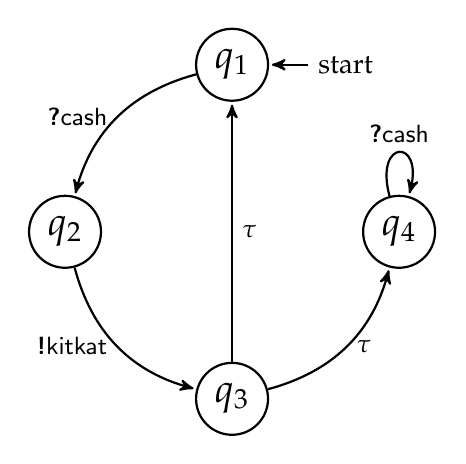
\begin{tikzpicture}[->,>=stealth',shorten >=1pt,auto,node distance=3cm,
                    thick,main
                    node/.style={circle,draw,font=\sffamily\Large\bfseries},
                    %initial text={   }
                    ] 
  \node[initial,initial where=right, main node] (1) [] {$q_1$};
  \node[main node] (2) [below left of=1] {$q_2$};
  \node[main node] (3) [below right of=2] {$q_3$};
  \node[main node] (4) [below right of=1] {$q_4$};

  \path[every node/.style={font=\sffamily\small}]
    (1) edge [bend right] node[left] {{\bfseries ?}cash} (2)
    (2) edge [bend right] node[left] {{\bfseries !}kitkat} (3)
    (3) edge node [right] {$\tau$} (1)
    (4) edge [loop above] node {{\bfseries ?}cash} (4)
    (3) edge [bend right] node[right] {$\tau$} (4);
\end{tikzpicture}
\end{center}
\end{wrapfigure}
In Model Based Testing (MBT) we express conformance via an \textit{Labeled
Transition System} (LTS). Because transition systems have a theoretical
background, information scientists are familiar with them. But also computer
scientists need a lot of knowledge to express conformance in the form of an LTS. 
In figure \ref{candymachine} we express a very abstract specification of what a candy
machine can do and cannot do in the form of an LTS.
\begin{enumerate}
  \item A candy machine starts in state $q_1$
  \item After the candy machine gets cash it must output a
  kitkat and go into state $q_2$
  \item Then it may either go back into state $q_1$ or it goes to state $q_4$
  \item In state $q_4$ it must not output a kitkat and only accept cash.
\end{enumerate}

In MBT we can derive test cases automatically from the LTS. That is why MBT
is one of the most advanced testing approaches nowadays. We can also exchange
the software product since our test cases do not rely on it, and test a bad
behaviour (e.g. ``do not explode'') on several products. 

\section*{Model Checking}
In contrast to testing Model Checking (MC) \textit{verifies} if a program
conforms. This means that we are not only ``almost certain'' that a program
conform - we are ``absolutely certain'' that a program conforms. Thus, if we
test a very critical programm, we can be certain that it does not malfunction.
Unfortunately this approach is not only very hard to implement, MC is sometimes
impossible to compute. In theory the model checking of a program could take much
more computation steps than there are atoms in the universe. Pioneering work was
done by E. M. Clarke for what he received the Turing Award. A keywork of
his work was defined checkable properties:
\begin{enumerate}
  \item Statements like ``Never do {\color{red}this}'' are called
  \textit{persistent properties}
  \item Statements like ``After doing {\color{red}this} you may do
  {\color{blue}that} never again'' are called \textit{liveness properties}
\end{enumerate}

It may be unclear that this is exactly the behaviour that we want to check, but
it can be shown that we can express every characterization of a program and
therefore making MC the ultimate tool for conformance checking. However MC does
still need a quite long time to compute even simple programs. 

%------------------------------------------------

\section*{Conclusion}
In this essay we have shown the difference between testing and verifying. 
Conformance checking is an important topic for the industry and therefore we
should think more about how to do it more efficient. On account of this we have
shown that we can do much better than Monkey Testing.

\bibliographystyle{unsrt}

\bibliography{../sample}

%----------------------------------------------------------------------------------------

\end{document}